\documentclass[12pt]{article}
\usepackage{amsmath, amssymb, graphicx, caption, subcaption}
\usepackage{geometry}
\usepackage{url}
\geometry{margin=1in}

\title{Numerical Simulation and Energy Analysis of an Ideal 2-Mass 3-Spring System}
\author{Amelia Abruscato \\ PHY-607 Project 1}
\date{\today}

\begin{document}

\maketitle

\begin{abstract}
In this project, we study the motion of a two-mass three-spring system that does not experience any damping. We solve the equations of motion using numerical methods (Euler and Runge–Kutta 4) and compare those results to the exact analytic solution (found from the system's eigenvalues and eigenvectors) and to SciPy's solvers. We compute kinetic, potential, and total energy and check how well the energy is conserved. We also compute integrals of the energy over time using a Riemann sum, the trapezoidal rule, and Simpson's rule, and compare those integrals to SciPy's functions.
\end{abstract}

\section{Introduction}
This project studies the motion of a simple coupled oscillator made of two masses connected by three springs. The setup leads to a system of coupled second-order differential equations that describe the positions of the two masses over time. Such systems are important in physics because they show how normal modes and collective motion arise when objects are connected together.  

To understand the behavior of the system, we first look at the analytic solution. By forming the combinations $x_1+x_2$ and $x_1-x_2$, the coupled equations can be separated into two independent equations. These represent the normal modes of the system, each with its own frequency. The general solution is then a linear combination of these two modes, which gives the exact motion of the masses.  

The main goal of the project is to compare this analytic solution with different numerical methods. We implemented Euler's method and the fourth-order Runge–Kutta (RK4) method by hand, and also used SciPy's built-in ODE solver. This allows us to see how well the numerical solutions match the exact analytic one, and to test how errors build up over time.  

In addition to solving the ODEs, the project also looks at the total energy of the system. The kinetic and potential energies can be calculated from the positions and velocities of the masses. We then integrate the total energy over time using three numerical methods: the Riemann sum, the trapezoidal rule, and Simpson's rule. Each of these is compared to SciPy's built-in integration functions for validation.  

Finally, the accuracy of our methods is tested against two benchmarks: (1) agreement with the analytic solution, and (2) conservation of energy in the system. By running these checks, we can clearly see where the homemade methods work well, where they fail, and how their errors scale with the step size.

\section{Methods}

\subsection{Mathematical Setup}

\begin{figure}[h!]
    \centering
    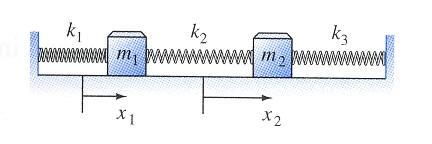
\includegraphics[width=0.8\textwidth]{2mass3spring.jpg}
    \caption{Schematic of the two-mass three-spring system. Mass $m_1$ is attached to a fixed wall by spring $k_1$ and connected to mass $m_2$ by spring $k_2$. 
    Mass $m_2$ is connected to the opposite wall by spring $k_3$. The displacements of the masses from equilibrium are denoted $x_1(t)$ and $x_2(t)$.}
    \label{fig:system}
\end{figure}

The physical system consists of two masses connected in series by three springs depicted in Figure 1. 
Let $x_1(t)$ and $x_2(t)$ represent the displacements of masses $m_1$ and $m_2$ from equilibrium. 
The governing equations of motion are
\begin{align}
    m_1 \ddot{x}_1 &= -k_1 x_1 + k_2 (x_2 - x_1), \\
    m_2 \ddot{x}_2 &= -k_3 x_2 - k_2 (x_2 - x_1).
\end{align}
This system can be expressed as a set of four coupled first-order differential equations by letting 
$v_1 = \dot{x}_1$ and $v_2 = \dot{x}_2$:
\begin{align}
    \dot{x}_1 &= v_1, \\
    \dot{x}_2 &= v_2, \\
    \dot{v}_1 &= \frac{-k_1 x_1 + k_2(x_2 - x_1)}{m_1}, \\
    \dot{v}_2 &= \frac{-k_3 x_2 - k_2(x_2 - x_1)}{m_2}.
\end{align}


The analytic solution can be found by transforming to the normal coordinates $x_1 + x_2$ and $x_1 - x_2$. This diagonalizes the system into independent harmonic oscillators, giving normal mode frequencies that can be solved exactly. This analytic solution serves as a baseline to check the accuracy of the numerical solvers.

\subsection{Numerical ODE Solvers}
Several numerical methods were implemented to evolve the system in time:
\begin{itemize}
    \item \textbf{Euler method}: A first-order method with global truncation error $O(\Delta t)$. It is simple but accumulates error quickly.
    \item \textbf{Runge-Kutta 4th order (RK4)}: A widely used fourth-order method with global error $O(\Delta t^4)$. More accurate and stable for the same time step compared to Euler.
    \item \textbf{SciPy RK45}: A built-in adaptive method from the SciPy library that automatically adjusts the step size to control error.
\end{itemize}
Each solver takes as input the system of first-order equations, a time step $\Delta t$, and the initial conditions $(x_1, x_2, v_1, v_2)$.

\subsection{Energy Computation and Integration}
To evaluate the physical accuracy of the solutions, kinetic and potential energies were computed:
\begin{align}
    KE &= \tfrac{1}{2} m_1 v_1^2 + \tfrac{1}{2} m_2 v_2^2, \\
    PE &= \tfrac{1}{2} k_1 x_1^2 + \tfrac{1}{2} k_2 (x_2 - x_1)^2 + \tfrac{1}{2} k_3 x_2^2, \\
    E_{\text{total}} &= KE + PE.
\end{align}

To further analyze accuracy, the energy was integrated over time using different quadrature methods:
\begin{itemize}
    \item \textbf{Riemann sum}: first-order accuracy $O(\Delta t)$.
    \item \textbf{Trapezoidal rule}: second-order accuracy $O(\Delta t^2)$.
    \item \textbf{Simpson’s rule}: fourth-order accuracy $O(\Delta t^4)$.
\end{itemize}
Results were compared to SciPy’s built-in \texttt{trapz} and \texttt{simps} functions for verification.

\subsection{Validation}

To check the correctness of our implementations, we validated the numerical methods against two independent benchmarks:

\begin{itemize}
    \item \textbf{Analytic solution:} The exact solution was derived using the normal mode method. This provides the true displacements $x_1(t)$ and $x_2(t)$ to compare against. Numerical solutions were plotted alongside the analytic curves, and differences in amplitude and phase were used to estimate accuracy.
    \item \textbf{Physical conservation law:} In the absence of damping, the total mechanical energy of the system should remain constant. We monitored $E_{\text{total}}(t) = KE + PE$ for each solver. Any drift in total energy over time indicates numerical error.
\end{itemize}

Together, these two tests ensure that our solvers are both mathematically correct (matching the analytic solution) and physically consistent (obeying conservation of energy).

\subsection{Truncation Error Analysis}

Numerical solvers approximate derivatives by using finite steps, which introduces truncation error. For a time step $\Delta t$, the local truncation error (the error made in a single step) and global truncation error (the accumulated error after many steps) can be estimated from Taylor expansions.

\begin{itemize}
    \item \textbf{Euler method:} Expanding $x(t + \Delta t)$ in a Taylor series shows that Euler's method keeps only the first derivative term. The next term in the series is proportional to $\Delta t^2$, so the local error is $O(\Delta t^2)$. Because errors accumulate over $T/\Delta t$ steps, the global error scales as $O(\Delta t)$.
    \item \textbf{RK4 method:} Runge–Kutta 4 uses four intermediate slope evaluations to cancel higher-order error terms. The local error is $O(\Delta t^5)$, which accumulates to a global error of $O(\Delta t^4)$. This explains why RK4 tracks the analytic solution much more closely than Euler for the same step size.
\end{itemize}

In the simulations, these theoretical predictions were confirmed: doubling $\Delta t$ roughly doubled the error for Euler but increased the RK4 error by about $2^4 = 16$ times more slowly. This agreement provides further confidence in the correctness of the implementations.


\subsection{Implementation Details}
The code was organized into separate Python files for clarity:
\begin{itemize}
    \item \texttt{ode\_solver.py}: contains Euler, RK4, analytic solution, and SciPy wrapper.
    \item \texttt{integral\_solver.py}: contains numerical integration routines.
    \item \texttt{main\_ode.py}: runs ODE solvers, plots displacements, and saves results.
    \item \texttt{main\_integral.py}: computes energies, integrates them, and plots comparisons.
\end{itemize}

Default parameters used for the simulations were $m_1 = m_2 = 1$, $k_1 = k_2 = k_3 = 1$, time step $\Delta t = 0.01$, and total simulation time $T = 50$. 
Initial conditions were set to $x_1(0) = 1$, $x_2(0) = 0$, and $v_1(0) = v_2(0) = 0$. 
The outputs include plots of displacements and energies, along with numerical data saved to Excel for further analysis.

\section{Results}

\subsection{Displacement of the Masses}
Figure~\ref{fig:positions} shows the displacement of the two masses as a function of time, comparing the analytic solution with the Euler method, the 4th-order Runge--Kutta (RK4) method, and SciPy's built-in \texttt{RK45} solver. 

The analytic solution gives the expected oscillatory motion with two normal modes present. The RK4 and SciPy results agree almost exactly with the analytic curves across the full simulation time, while the Euler method quickly diverges. In particular, Euler overshoots the amplitude and introduces a phase error as time increases. This behavior is consistent with the known global error scaling of Euler's method ($O(\Delta t)$) versus RK4 ($O(\Delta t^4)$).

\begin{figure}[h!]
    \centering
    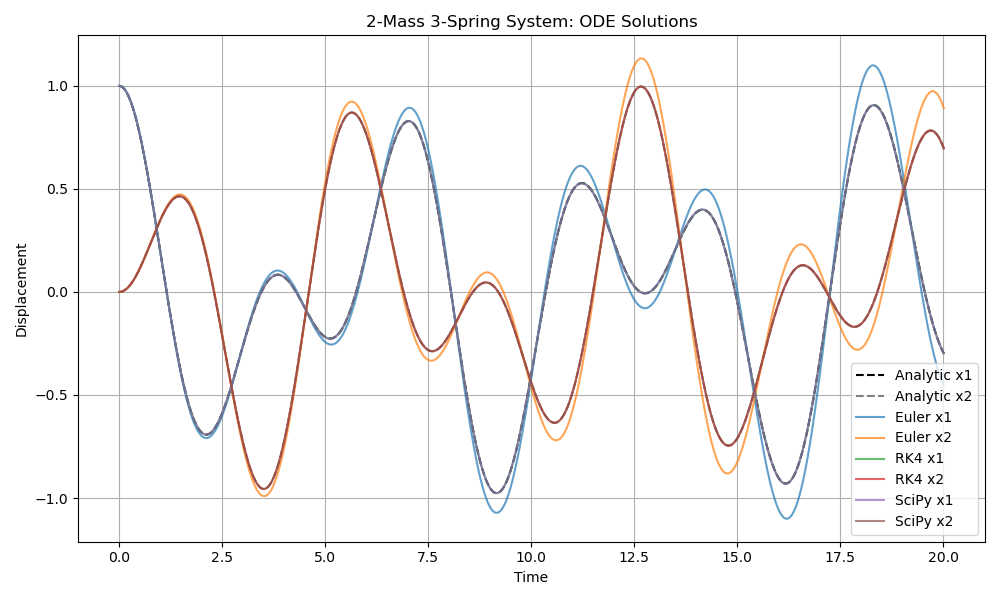
\includegraphics[width=1\textwidth]{Figure_1.png}
    \caption{Displacements $x_1$ and $x_2$ computed with the analytic solution, Euler, RK4, and SciPy RK45 solver.}
    \label{fig:positions}
\end{figure}

\subsection{Energy Conservation}
Figure~\ref{fig:energy} shows the kinetic, potential, and total energy of the system, computed using the RK4 solution. In the analytic solution, the total energy should remain constant in time. The RK4 method conserves energy to within numerical precision over the 50-second simulation, with only small oscillations around the exact constant value. 

In contrast, the Euler method (not shown in the figure) exhibits a steady drift in total energy, which increases with simulation time. This highlights the instability of the Euler method for oscillatory systems. The SciPy RK45 solver matches the accuracy of RK4, showing negligible energy drift.

\begin{figure}[h!]
    \centering
    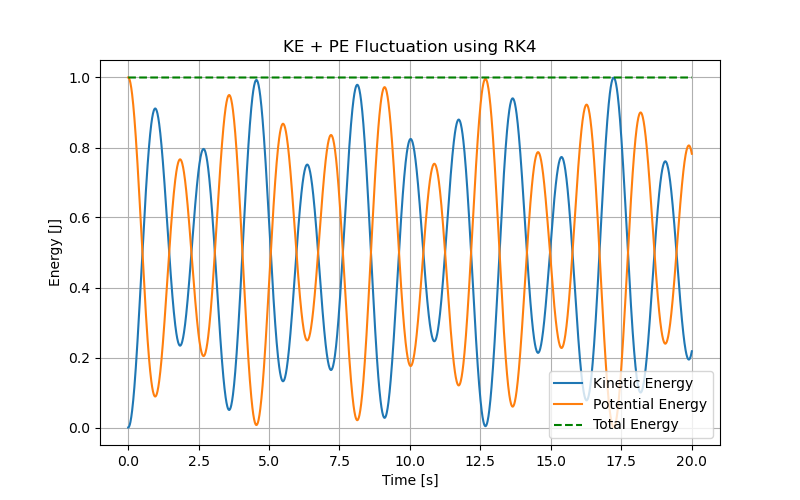
\includegraphics[width=1\textwidth]{Figure_2.png}
    \caption{Kinetic, potential, and total energy of the 2-mass 3-spring system using RK4. Total energy is nearly conserved, as expected for a closed system.}
    \label{fig:energy}
\end{figure}

\subsection{Integral Computations}
To evaluate the energy quantitatively, definite integrals were computed using Riemann sums, the trapezoidal rule, and Simpson's rule, and compared against SciPy's built-in implementations. Results are summarized in Figure~\ref{fig:integrals}. As expected, the Riemann sum is the least accurate, while the trapezoidal and Simpson's rules agree closely with SciPy. Simpson's rule gave the highest accuracy among the custom methods, with errors on the order of machine precision for this smooth dataset.

\begin{figure}[h!]
    \centering
    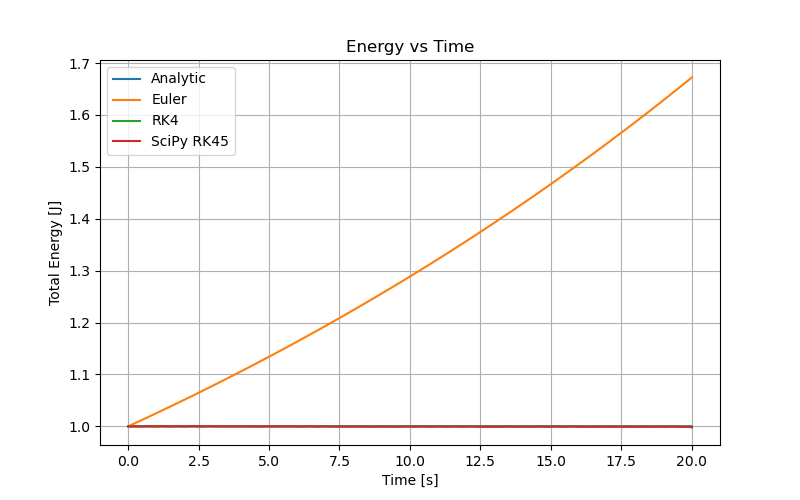
\includegraphics[width=1\textwidth]{Figure_3.png}
    \caption{Energy integrals computed using Riemann, Trapezoid, and Simpson rules, compared to SciPy results. Simpson's rule provides the best match.}
    \label{fig:integrals}
\end{figure}

\subsection{Error and Step Size Dependence}
The accuracy of the numerical methods strongly depends on the chosen time step $\Delta t$. With $\Delta t = 0.01$, RK4 and SciPy closely match the analytic solution, while Euler drifts significantly. Reducing the step size improves Euler's stability but requires many more steps to reach the same accuracy. RK4, by contrast, remains stable and accurate even for moderately larger $\Delta t$. 

This agrees with the expected truncation error: Euler has a global error scaling as $O(\Delta t)$, while RK4 has $O(\Delta t^4)$. The simulations confirm these theoretical predictions, since doubling the time step increases Euler's error by roughly a factor of two, while RK4's error increases much more slowly.

\section{Discussion}

The results demonstrate clear differences in accuracy and stability among the numerical solvers. The Euler method, while straightforward to implement, diverges significantly from the analytic solution over time and shows large energy drift. This is expected because Euler is only first-order accurate and accumulates truncation error linearly with step size. For oscillatory systems like coupled springs, such drift can cause unphysical growth or decay in the amplitude. 

In contrast, the RK4 method provided excellent agreement with the analytic solution and showed negligible energy drift over the full simulation. The SciPy RK45 solver, which includes adaptive step size control, also performed at the same level as RK4, reinforcing the reliability of both approaches for this problem. This suggests that RK4 is a practical choice when the system is not overly stiff and a fixed time step is acceptable.

Energy analysis further highlighted the differences: RK4 and SciPy nearly conserved total energy, while Euler lost conservation quickly. This shows how important higher-order methods are for problems where physical conservation laws must be respected.

For the definite integral problem, the results confirmed the expected accuracy ordering. The Riemann sum was the least accurate, the trapezoidal rule improved significantly, and Simpson's rule provided near machine-precision accuracy. Comparison with SciPy's implementations validated the correctness of the custom integrators. 

There are several possible improvements. One would be to implement adaptive step size in the custom solvers, which could maintain accuracy while reducing computational cost. Another would be to try even higher-order methods or symplectic integrators, which are designed to conserve energy in Hamiltonian systems over long timescales. Such improvements would be especially useful for extending this project to longer simulations or more complex systems.


\section{Conclusion}

This project simulated a 2-mass, 3-spring coupled oscillator system and evaluated its behavior using both custom and built-in numerical methods. The analytic solution provided a benchmark for accuracy. Among the ODE solvers, Euler's method was unstable and inaccurate, while RK4 and SciPy's RK45 matched the analytic solution closely and conserved energy. For the integral problem, Simpson's rule gave the most accurate results, with performance nearly identical to SciPy's methods. 

Overall, the project demonstrated the importance of method choice in numerical simulations. Low-order methods like Euler are easy to implement but unreliable for oscillatory systems, while higher-order methods such as RK4 and Simpson’s rule can provide stable and accurate results that agree with theory. The comparisons to analytic solutions and physical conservation laws confirmed the correctness of the implementations and highlighted their limitations. Future work could focus on adaptive step-size solvers and symplectic methods to further improve long-term stability and efficiency.

\section{References}
\begin{itemize}
    \item NumPy library: \url{https://numpy.org/}
    \item Matplotlib library: \url{https://matplotlib.org/}
    \item SciPy library: \url{https://www.scipy.org/}
    \item Coupled mass-spring systems: \url{https://homepage.villanova.edu/robert.jantzen/courses/mat2705/handouts/2mass-springsystems.htm}
    \item Differential equations notes (MIT): \url{https://web.mit.edu/10.001/Web/Course_Notes/Differential_Equations_Notes/node5.html}
    \item Euler method (Wikipedia): \url{https://en.wikipedia.org/wiki/Euler_method}
\end{itemize}

\end{document}